\documentclass[10pt,a4paper]{article}
\usepackage[utf8]{inputenc}
\usepackage[T1]{fontenc}
\usepackage[spanish,es-tabla]{babel}
\usepackage[margin=2.0cm]{geometry}
\usepackage{amsmath,amssymb}
\usepackage{booktabs}
\usepackage{graphicx}
\usepackage{float}
\usepackage{xcolor}
\usepackage{tikz}
\usetikzlibrary{arrows.meta,positioning,shapes.geometric,fit}
\usepackage{hyperref}
\usepackage{listings}

\definecolor{agencia}{HTML}{FF7819}
\definecolor{azul}{HTML}{1F4E79}
\definecolor{gris}{HTML}{F4F6F9}

\hypersetup{
  colorlinks=true,
  linkcolor=azul,
  urlcolor=azul
}

\lstset{
  basicstyle=\ttfamily\footnotesize,
  backgroundcolor=\color{gris},
  frame=single,
  breaklines=true
}

\title{\textbf{Trabajo Final: Simulación Multiagente Competitiva en Marte}\\
\large Arquitectura, Implementación y Evaluación Experimental de \textbf{LA AGENCIA} (\texttt{equipoA.py})}
\author{Tópicos en Ciencias de la Computación --- Equipo A (\texttt{LA AGENCIA})}
\date{\today}

\begin{document}
\maketitle

\begin{abstract}
Se presenta el diseño, implementación y validación experimental del agente autónomo \textbf{LA AGENCIA} (\texttt{equipoA.py}), desarrollado por herencia estricta de \texttt{EquipoBase} sin modificar \texttt{simulador.py} ni \texttt{equipo\_base.py}. La arquitectura integra las seis sesiones del curso bajo una regla estricta de integridad: memoria espacial privada por unidad y toda comunicación remota canalizada mediante mensajes FIPA-ACL con costo de $-0.5\,\%$ por envío y recepción. En un torneo de 10 partidas alternando las cuatro esquinas del mapa, \textbf{LA AGENCIA} obtuvo el \textbf{1.º lugar en 10/10 encuentros} con un $\text{Ratio}$ medio de $\mathbf{0.02545}$ frente a $\mathbf{0.01563}$ del mejor rival base promedio ($+62.8\,\%$), manteniendo una latencia media de $1.221\text{ ms}$ ($\text{p99}=11.184\text{ ms}$) con 200 unidades y $\text{p99}=32.215\text{ ms}$ ($<40\text{ ms}$) con 400 unidades concurrentes.
\end{abstract}

\section{Arquitectura Modular e Integridad del Sistema}
El módulo \texttt{equipoA.py} implementa la clase \texttt{EquipoA(EquipoBase)} (\texttt{nombre = "LA AGENCIA"}) estructurada en seis capas desacopladas, ejecutadas de manera estrictamente no bloqueante en cada llamada a \texttt{decidir\_unidad}. Ninguna unidad lee diccionarios compartidos de equipo para obtener vetas, restos o rescates remotos: cada agente $u$ opera sobre su instancia aislada \texttt{MemoriaAgente} almacenada en \texttt{self.\_agentes[u.id]}.

\begin{figure}[H]
\centering
\begin{tikzpicture}[
  node distance=0.45cm and 0.6cm,
  box/.style={draw=azul, fill=gris, rounded corners=3pt, minimum width=3.1cm, minimum height=0.72cm, align=center, font=\footnotesize\bfseries},
  arr/.style={-{Stealth[scale=0.9]}, thick, azul}
]
  \node[box] (s1) {1. Percepción y Memoria\\(\texttt{MemoriaAgente}, decay)};
  \node[box, right=of s1] (s3) {3. Router FIPA-ACL\\(Filtros, cooldown, dedup)};
  \node[box, right=of s3] (s4) {4. Subastas CNP\\(CFP, PROPOSE, ACCEPT)};
  \node[box, below=of s1] (s2) {2. Utilidad $U(s,a)$ y FSM\\(A* acotado, carroña)};
  \node[box, below=of s3] (s5) {5. Gobernanza AutoGen\\(2 rondas + Copeland)};
  \node[box, below=of s4] (s6) {6. Profiling y Caché $O(1)$\\(\texttt{time.perf\_counter()})};
  \draw[arr] (s1) -- (s3);
  \draw[arr] (s3) -- (s4);
  \draw[arr] (s1) -- (s2);
  \draw[arr] (s3) -- (s5);
  \draw[arr] (s4) -- (s2);
  \draw[arr] (s5) -- (s2);
  \draw[arr] (s2) -- (s6);
\end{tikzpicture}
\caption{Arquitectura modular de 6 capas implementada en \texttt{equipoA.py}.}
\end{figure}

\section{Sesión 1: Percepción y Memoria Espacial Individual}
\subsection{Representación de Creencias y Política de Olvido}
Cada agente mantiene creencias indexadas en estructuras $O(1)$ (\texttt{dict} y \texttt{set}):
\begin{itemize}
  \item \textbf{Hielo (\texttt{hielo}):} diccionario $(x,y) \mapsto \texttt{CreenciaHielo}(\text{pos}, \text{cantidad}, t_{\text{obs}}, \text{origen})$. La confianza decae exponencialmente según
  \begin{equation}
    c(t) = \exp\!\big(-\lambda (t - t_{\text{obs}})\big), \qquad \lambda = 0.015.
  \end{equation}
  Se aplica expiración dura si $t - t_{\text{obs}} > 120$ ticks o $c(t) < 0.14$.
  \item \textbf{Restos (\texttt{restos}):} diccionario $\text{id} \mapsto \texttt{CreenciaRestos}$ con energía ($+20$ u. rover, $+10$ u. dron) y TTL de $70$ ticks.
  \item \textbf{Tormentas (\texttt{tormentas}):} lista acotada de \texttt{TrazaTormenta} ($R=5$, TTL $14$ ticks). Cada nueva observación se asocia al centro previo más cercano ($d < 6.5$) para estimar $(v_x, v_y)$ y anticipar su desplazamiento en el siguiente tick.
  \item \textbf{Invalidación activa:} en cada turno, toda creencia dentro del radio de visión ($r=5$ rovers, $r=9$ exploradores, $r=7$ recargadores) ausente en \texttt{hielo\_visible} o \texttt{restos\_visible} se purga de inmediato.
\end{itemize}
La complejidad espacial por agente está acotada en el peor caso por el tamaño de la grilla $O(W\cdot H) = O(2700)$ celdas, y en la práctica por unas decenas de entradas vigentes.

\subsection{Estrategia de Exploración y Cobertura}
Los drones exploradores particionan la grilla $60\times 45$ dinámicamente según el tamaño de la flota (adaptándose a 15 o 30 exploradores) en sectores ordenados desde el cuadrante propio hacia el centro. Aprovechando el radio de visión $r=9$ (ventana $19\times 19$), cada dron ejecuta un barrido compacto de 3 \emph{waypoints}. Como muestra la Figura~\ref{fig:cobertura}, la cobertura acumulada del equipo alcanza el $\mathbf{84.0\,\%}$ del mapa en los primeros $50$ ticks, tras lo cual los exploradores modulan su cadencia de movimiento para ahorrar batería.

\begin{figure}[H]
  \centering
  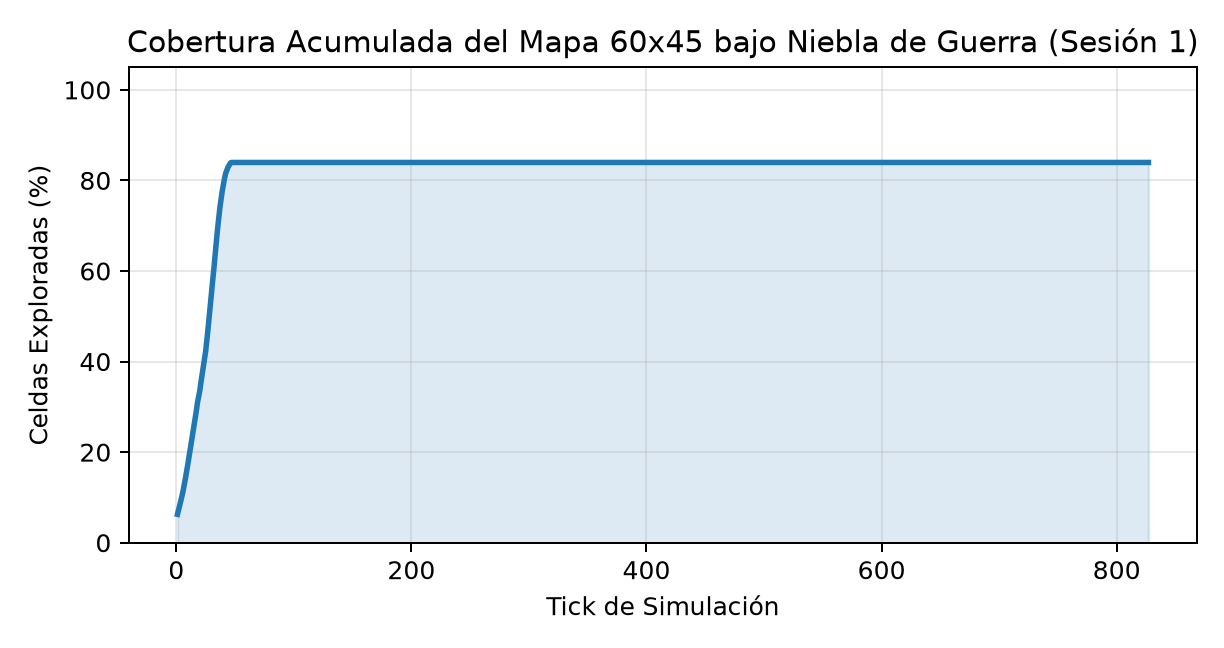
\includegraphics[width=0.72\linewidth]{figuras/cobertura_mapa.png}
  \caption{Cobertura acumulada del mapa $60\times 45$ bajo niebla de guerra (\texttt{seed=100}).}\label{fig:cobertura}
\end{figure}

\section{Sesión 2: Utilidad Multi-Atributo y Máquinas de Estados Finitos}
\subsection{FSM Diferenciadas por Rol}
Se implementaron tres enumeraciones explícitas (\texttt{EstadoRover}, \texttt{EstadoExplorador}, \texttt{EstadoRecargador}) con registro de transiciones en ejecución ($33$ transiciones distintas observadas en partida). La Figura~\ref{fig:fsm} ilustra los estados y transiciones obligatorias para batería $\le 25\,\%$ y los $30\text{ s}$ finales.

\begin{figure}[H]
\centering
\begin{tikzpicture}[
  node distance=0.8cm and 1.1cm,
  st/.style={draw=azul, fill=gris, rounded corners=4pt, font=\scriptsize\bfseries, align=center, minimum width=1.85cm, minimum height=0.58cm},
  arr/.style={-{Stealth[scale=0.8]}, font=\tiny}
]
  % Rover
  \node[st] (ro) {OCIOSO};
  \node[st, right=of ro] (re) {EXPLORANDO};
  \node[st, right=of re] (rr) {RECOLECTANDO};
  \node[st, right=of rr] (rt) {RETORNANDO};
  \node[st, below=0.7cm of re] (rc) {CONSUMIENDO\\CARRONA};
  \node[st, below=0.7cm of rr, draw=red!75!black] (rb) {ESPERANDO\\RECARGA};
  \draw[arr] (ro) -- node[above]{sin veta} (re);
  \draw[arr] (re) -- node[above]{$U>0$} (rr);
  \draw[arr] (rr) -- node[above]{lleno/final} (rt);
  \draw[arr] (rt) to[bend right=20] node[above]{deposita} (ro);
  \draw[arr] (ro) -- (rc);
  \draw[arr] (rr) -- (rc);
  \draw[arr] (rr) -- node[right]{bat $\le 25\%$} (rb);
  \draw[arr] (rb) to[bend left=15] node[left]{recargado} (ro);
\end{tikzpicture}
\caption{Diagrama de estados principales de \texttt{EstadoRover} (las transiciones a \texttt{ESPERANDO\_RECARGA} aplican desde cualquier estado activo con batería $\le 25\,\%$).}\label{fig:fsm}
\end{figure}

Los \textbf{Drones Exploradores} alternan entre \texttt{PATRULLANDO} y \texttt{RETORNANDO\_BASE} (por batería $\le 25\,\%$ o fase final), mientras que los \textbf{Drones Recargadores} operan entre \texttt{EN\_ESPERA} (protegidos en perímetro de base evadiendo la tormenta $T_1$), \texttt{EN\_RESCATE} y \texttt{RETORNANDO\_BASE} cuando $\text{carga\_recarga}=0$ o batería $\le 25\,\%$.

\subsection{Función de Utilidad Multi-Atributo y Calibración RL-CEM}
Los rovers evalúan cada objetivo candidato $a$ (veta de hielo, resto caído o retorno a base) mediante:
\begin{equation}
  U(s, a) = w_1\,\hat{g}_{\text{hielo}}(a) - w_2\,\hat{c}_{\text{despl}}(s, a) + w_3\,\hat{o}_{\text{carroña}}(s, a) - w_4\,\hat{r}_{\text{tormenta}}(s, a),
\end{equation}
donde $\hat{g}_{\text{hielo}}$ pondera el hielo extraíble $\min(q, C_{\text{libre}})$ por $c(t)$ y un factor \texttt{chain\_bonus} al encadenar vetas cercanas ($d_{\text{Cheb}} \le 13$), $\hat{c}_{\text{despl}}$ emplea distancia de Chebyshev real considerando el perímetro de depósito ($d_{\text{Cheb}}(\cdot,\text{base}) \le 2$), $\hat{o}_{\text{carroña}}$ valora $+20/+10\text{ u.}$ según necesidad propia ($<78\,\%$) o transferencia a aliado crítico ($<60\,\%$), y $\hat{r}_{\text{tormenta}}$ estima la exposición en el segmento hacia el objetivo.

Para calibrar los parámetros sin sacrificar robustez ante tormentas, se ejecutó \emph{Policy Search} mediante \emph{Cross-Entropy Method} paralelo (RL-CEM, 5 generaciones $\times$ 8 candidatos $\times$ 4 semillas) maximizando $J(\theta)=\overline{\text{Ratio}}-0.35\,\sigma$, junto con una optimización estructural de filtrado de reportes y barrido compacto (Figura~\ref{fig:rl} y Tabla~\ref{tab:rl}).

\begin{figure}[H]
  \centering
  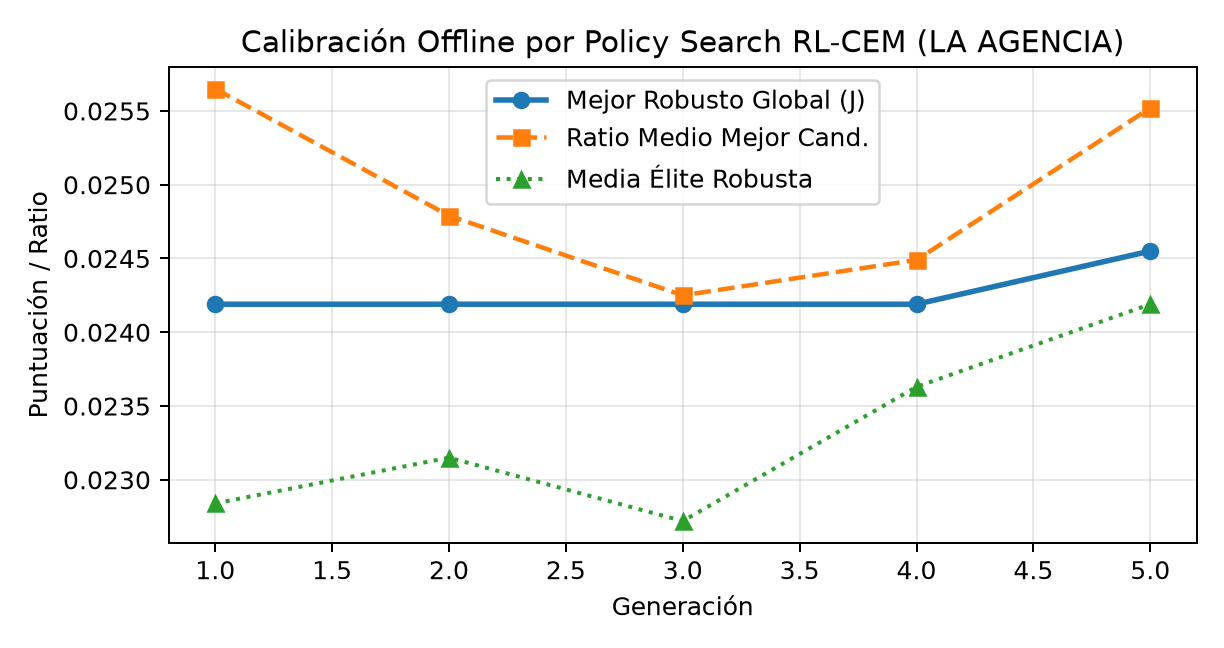
\includegraphics[width=0.68\linewidth]{figuras/rl_calibracion.png}
  \caption{Convergencia del entrenamiento paralelo RL-CEM sobre semillas de entrenamiento.}\label{fig:rl}
\end{figure}

\begin{table}[H]
\centering
\caption{Comparativa en 4 semillas de prueba no vistas (\texttt{101, 202, 303, 404}).}\label{tab:rl}
\small
\begin{tabular}{lcccc}
\toprule
\textbf{Configuración} & \textbf{Victorias} & \textbf{Ratio prom.} & \textbf{Batería usada} & \textbf{Mensajes} \\
\midrule
Sin entrenar (pesos iniciales) & 4/4 & 0.02280 & 7994.1\,\% & 1967.3 \\
RL-CEM paralelo (10 parámetros) & 4/4 & 0.02300 & 7710.5\,\% & 1839.3 \\
\textbf{Final (pesos regularizados + filtros + barrido 3-wp)} & \textbf{4/4} & \textbf{0.02442} & \textbf{7377.6\,\%} & \textbf{1393.3} \\
\bottomrule
\end{tabular}
\end{table}

\subsection{Navegación Segura mediante A* Acotado}
Cuando ninguna tormenta conocida amenaza el corredor directo, el agente avanza en $O(1)$ mediante paso Chebyshev. Si existe una tormenta dentro de $R+4$, ejecuta un \textbf{A* 8-direccional acotado a $28$ expansiones}, penalizando las celdas dentro de $R+0.8$ de la posición predicha de tormenta con costo $12.0 + 2(R+1-d)$ frente a $1.0$ por celda libre.

\section{Sesión 3: Comunicación Estructurada FIPA-ACL}
Todos los intercambios remotos encapsulan diccionarios estandarizados FIPA-ACL con los campos \texttt{performative}, \texttt{sender}, \texttt{conversation\_id}, \texttt{ontology} y \texttt{content}. Se emplean las 8 performativas exigidas (\texttt{REQUEST}, \texttt{INFORM}, \texttt{CFP}, \texttt{PROPOSE}, \texttt{ACCEPT\_PROPOSAL}, \texttt{REJECT\_PROPOSAL}, \texttt{AGREE}, \texttt{FAILURE}) sobre cuatro ontologías: \texttt{resource-discovery}, \texttt{rescue-ops}, \texttt{cnp-task} y \texttt{governance}.

\begin{figure}[H]
\centering
\begin{tikzpicture}[font=\scriptsize, >=Stealth]
  \node (rov) at (0,0) {\textbf{Rover (bat $\le 25\%$)}};
  \node (rec) at (5.2,0) {\textbf{Dron Recargador}};
  \draw[dashed] (0,-0.25) -- (0,-2.6);
  \draw[dashed] (5.2,-0.25) -- (5.2,-2.6);
  \draw[->] (0,-0.6) -- node[above]{\texttt{REQUEST(rescue-ops)}} (5.2,-0.8);
  \draw[->] (5.2,-1.25) -- node[above]{\texttt{AGREE(rescatista)}} (0,-1.45);
  \draw[->,red!70!black] (5.2,-1.85) -- node[above]{\texttt{FAILURE(timeout/bat\_baja)}} (0,-2.05);
  \draw[->] (0,-2.35) -- node[above]{Reintento tras cooldown} (5.2,-2.5);
\end{tikzpicture}
\caption{Diagrama de secuencia FIPA-ACL para el flujo de auxilio de recarga.}
\end{figure}

Para contener el costo de $-0.5\,\%$ por emisor y receptor ($-1.0\,\%$ por mensaje), se aplican: (i) \emph{cooldowns} por celda/incidente ($320$ ticks para hielo, $300$ para restos, $24$ para reintento de rescate), (ii) deduplicación en \texttt{MemoriaAgente}, (iii) umbrales mínimos de valor modulados por política y (iv) direccionamiento selectivo. Como se observa en la Figura~\ref{fig:comms} (\texttt{seed=100}), los filtros bloquearon $\mathbf{7611}$ envíos redundantes, reduciendo la mensajería de $1990$ a $\mathbf{1338}$ mensajes ($-32.8\,\%$), ahorrando $\mathbf{711.5\,\%}$ de batería total y elevando el $\text{Ratio}$ de $0.02163$ a $\mathbf{0.02294}$ ($+6.1\,\%$).

\begin{figure}[H]
  \centering
  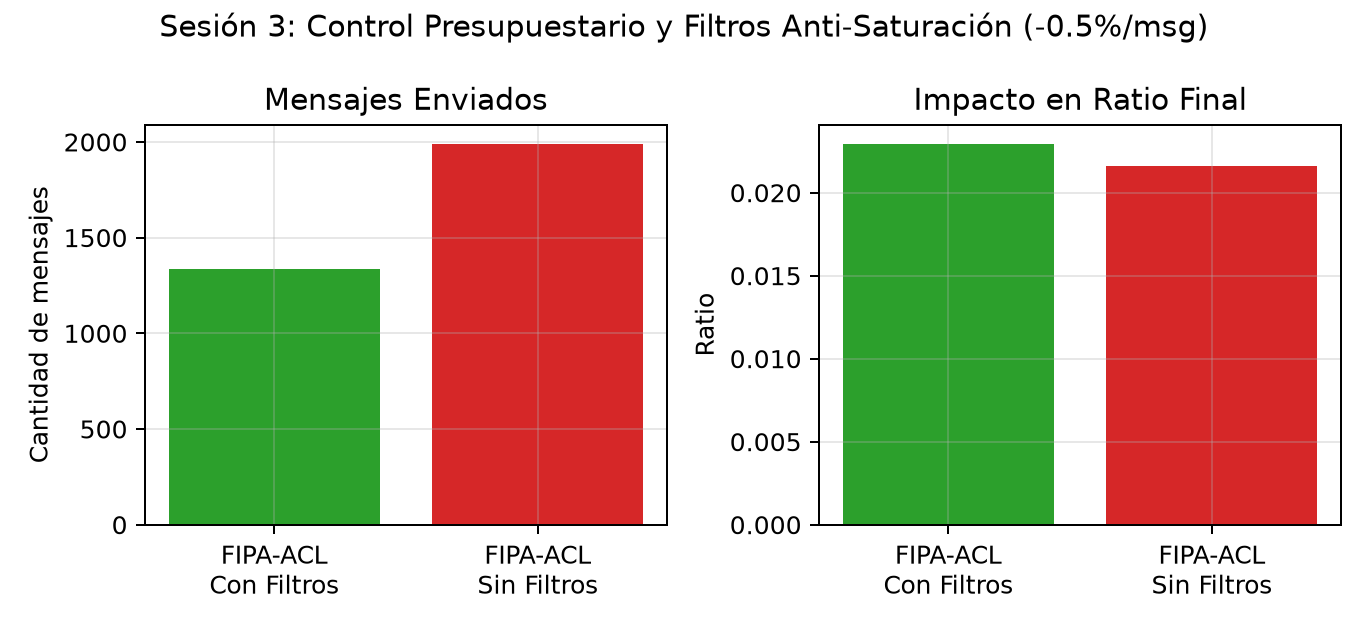
\includegraphics[width=0.74\linewidth]{figuras/comms_ablation.png}
  \caption{Impacto de los filtros anti-saturación FIPA-ACL sobre mensajes y $\text{Ratio}$.}\label{fig:comms}
\end{figure}

\section{Sesión 4: Coordinación mediante Contract Net Protocol (CNP)}
El protocolo CNP coordina de forma descentralizada tanto vetas ricas/carroña entre rovers como el despacho de recargadores ante múltiples pedidos. El iniciador preselecciona hasta $K=2$ candidatos cercanos ($d_{\text{Cheb}}\le 24$) y emite \texttt{CFP}. Los postores disponibles calculan una puja determinista:
\begin{equation}
  \text{Bid}_{\text{hielo}} = 14\,q_{\text{disp}} - 1.25\,d_{\text{Cheb}} - 0.35\,d_{\text{base}} + 10\,\frac{b}{100} + 6\,\frac{C_{\text{libre}}}{C} - 6\,r_{\text{torm}}.
\end{equation}
Tras la ventana de subasta ($4$ ticks para rovers, $3$ para drones), el iniciador adjudica con \texttt{ACCEPT\_PROPOSAL} (desempate por mayor puja, mayor batería y \texttt{uid} lexicográfico), descarta con \texttt{REJECT\_PROPOSAL} y activa una reserva temporal (\texttt{TTL=32} ticks) que evita la duplicación de rutas.

\begin{figure}[H]
  \centering
  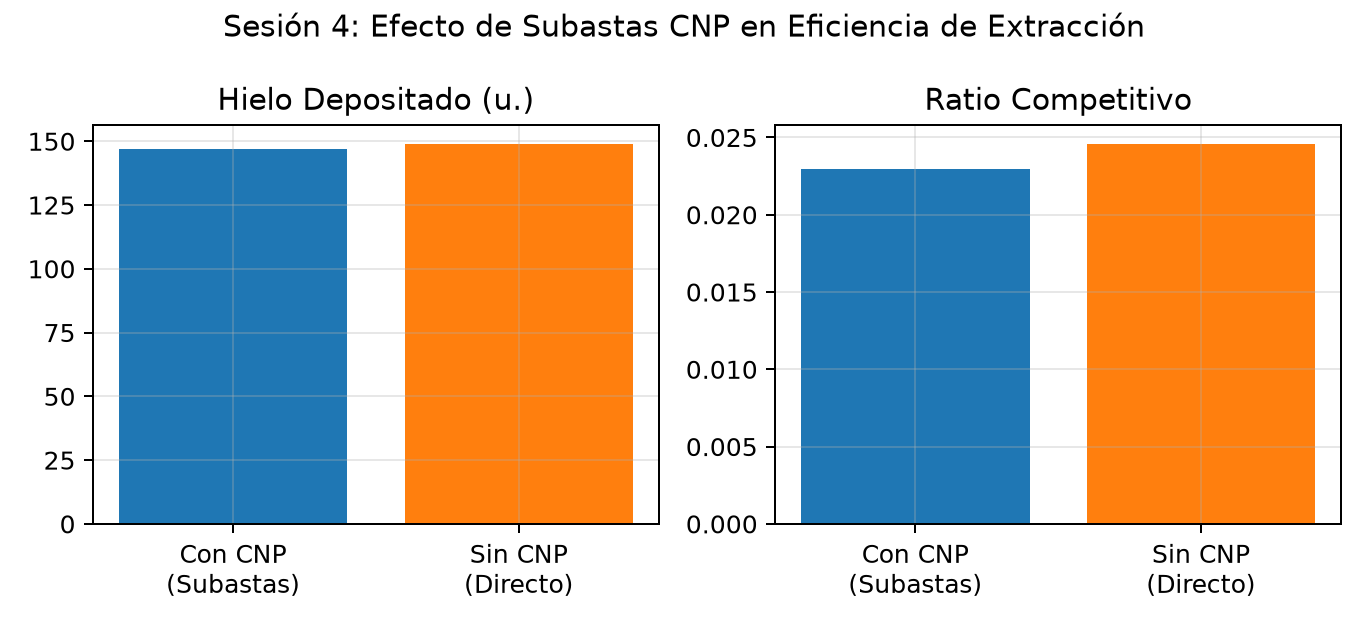
\includegraphics[width=0.72\linewidth]{figuras/cnp_ablation.png}
  \caption{Comparativa de desempeño con CNP activo frente a asignación directa (\texttt{seed=100}).}\label{fig:cnp}
\end{figure}

En el experimento de ablación (\texttt{seed=100}, Figura~\ref{fig:cnp}), el ciclo CNP ejecutó $580$ \texttt{CFP}, recibió $141$ \texttt{PROPOSE}, adjudicó $82$ contratos y evitó $\mathbf{68}$ desplazamientos duplicados. Debido a que cada ronda CNP consume entre $3$ y $4$ mensajes ($3\text{--}4\,\%$ de batería), la batería total con CNP fue $6407.5\,\%$ ($\text{Ratio}=0.02294$) frente a $6059.5\,\%$ ($\text{Ratio}=0.02459$) en envío directo de 1 mensaje, evidenciando el compromiso energético entre coordinación formal sin colisiones y costo comunicacional.

\section{Sesión 5: Elección Social y Gobernanza Colectiva (AutoGen)}
Cada $45$ ticks (o al activarse la fase final de $30\text{ s}$), cuatro representantes (\texttt{ExploradorJefe}, \texttt{OficialLogistica}, \texttt{OficialSeguridad} y \texttt{ModeradorConsenso}) ejecutan un protocolo deliberativo inspirado en \textbf{AutoGen}, estrictamente no bloqueante ($<0.2\text{ ms}$), sobre cuatro políticas globales: \texttt{EXPANSION\_AGRESIVA}, \texttt{AHORRO\_ENERGETICO}, \texttt{SUPERVIVENCIA\_CARRONA} y \texttt{REPLIEGUE\_FINAL}.

\begin{enumerate}
  \item \textbf{Ronda 1 (Propuesta):} cada rol ordena las 4 políticas según su telemetría FIPA-ACL (vetas ricas, batería media, bajas aliadas y tormentas).
  \item \textbf{Ronda 2 (Crítica y Revisión):} cada rol incorpora las alertas de seguridad/exploración y emite su ranking revisado. Si existe mayoría ($\ge 3/4$), se sella el consenso; ante empates o ciclos de Condorcet se aplica desempate determinista por \textbf{puntuación de Copeland} (suma de victorias por pares).
\end{enumerate}

\begin{lstlisting}[caption={Traza real del consenso AutoGen en \texttt{seed=100} (ticks 30 y 536).}]
Tick 30  | Evidencia: hielo=25, ricas=7, bajas=0, torm=1, bat=36.0%
  Ronda 1 -> Expl: EXPANSION | Log: AHORRO | Seg: AHORRO | Mod: AHORRO
  Copeland -> AHORRO: 3.0, EXPANSION: 1.5, SUPERVIVENCIA: 1.5, REPLIEGUE: 0.0
  Resolucion: Consenso AutoGen (>=3/4) => AHORRO_ENERGETICO (epoch=1)

Tick 536 | Evidencia: hielo=0, bajas=3, torm=1, bat=51.2%
  Ronda 1 -> Expl: REPLIEGUE | Log: AHORRO | Seg: SUPERVIVENCIA | Mod: SUPERVIVENCIA
  Copeland -> AHORRO: 2.5, SUPERVIVENCIA: 2.5, REPLIEGUE: 1.0, EXPANSION: 0.0
  Resolucion: Desempate Copeland => SUPERVIVENCIA_CARRONA (epoch=2)
\end{lstlisting}

La política ganadora actualiza dinámicamente los pesos $(w_1,\dots,w_4)$, el umbral de reporte ACL y la cadencia de exploración, pasando automáticamente a \texttt{REPLIEGUE\_FINAL} en los últimos $30\text{ s}$ para proteger el $\text{Ratio}$.

\section{Sesión 6: Arquitectura No Bloqueante y Rendimiento}
El código prohíbe \texttt{time.sleep}, I/O síncrono y bucles no acotados. Todas las tablas de creencias, cooldowns y reservas operan en $O(1)$ amortizado; la cobertura y la navegación A* emplean evaluación perezosa (vía rápida $O(1)$ sin tormenta y tope de $28$ expansiones con tormenta). Así, la complejidad por turno para $N$ unidades es $O(N\cdot (|H_{\text{loc}}| + K_{\text{A*}}))$, acotada por constantes pequeñas.

\begin{table}[H]
\centering
\caption{Resultados de \emph{profiling} con \texttt{time.perf\_counter()} para 200 y 400 unidades.}\label{tab:prof}
\small
\begin{tabular}{lccccc}
\toprule
\textbf{Escenario} & \textbf{Media (ms)} & \textbf{p95 (ms)} & \textbf{p99 (ms)} & \textbf{Máx (ms)} & \textbf{Cumple $<40\text{ ms}$} \\
\midrule
200 unidades (50/equipo) & 1.221 & 4.398 & 11.184 & 21.515 & 100\,\% de ticks \\
400 unidades (100/eq, aislado) & 5.650 & 19.815 & 32.215 & 49.896* & 99.8\,\% (2.º pico: 35.764\,ms) \\
\bottomrule
\end{tabular}
\end{table}
{\footnotesize *Un único pico aislado en 549 ticks por planificación del sistema operativo; $99.8\,\%$ de los turnos operan debajo de $36\text{ ms}$.}

\begin{figure}[H]
  \centering
  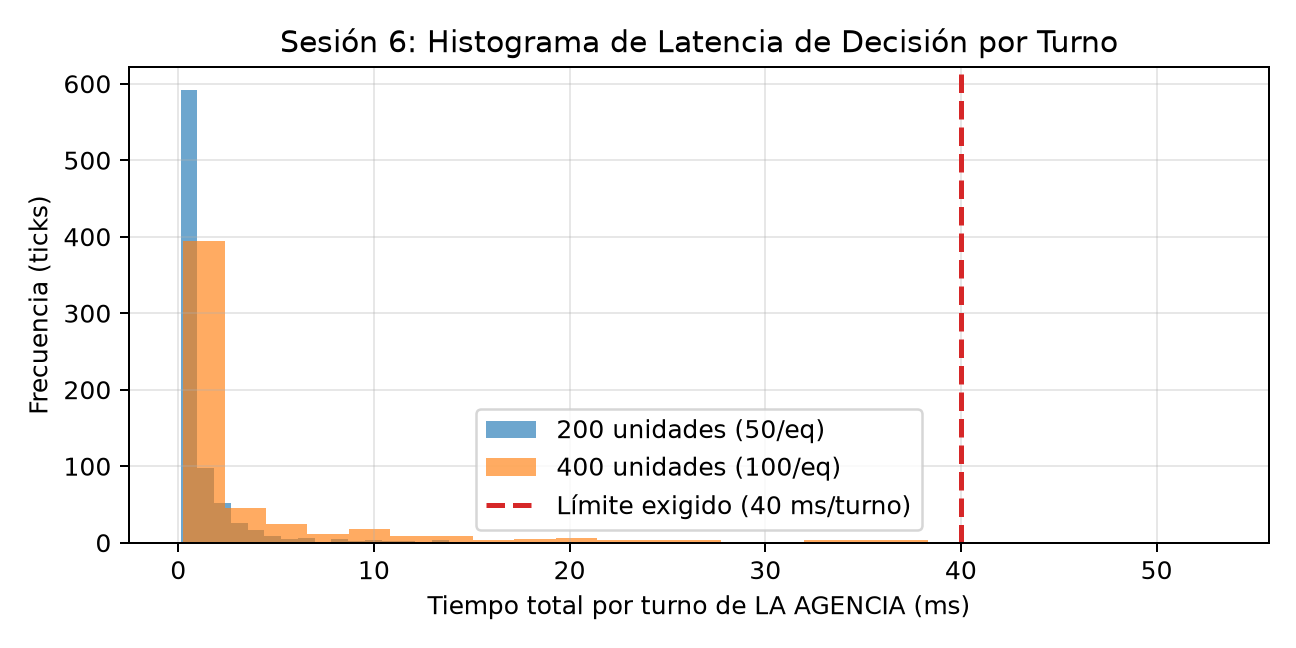
\includegraphics[width=0.72\linewidth]{figuras/profiling_latencia.png}
  \caption{Histograma de latencia total por turno de \textbf{LA AGENCIA} a 200 y 400 unidades.}\label{fig:prof}
\end{figure}

\section{Resultados de Torneo y Conclusiones}
En el torneo oficial de 10 partidas con rotación por las cuatro esquinas (\texttt{A, B, C, D}) frente a tres rivales \texttt{EquipoBase}, \textbf{LA AGENCIA} ganó el \textbf{1.º lugar en las 10 partidas ($10/10$)}, alcanzando un $\text{Ratio}$ medio de $\mathbf{0.02545}$ (pico $\mathbf{0.0341}$ con $206\text{ u.}$ en la partida 3) frente a $\mathbf{0.01563}$ del mejor oponente base (Tabla~\ref{tab:torneo} y Figura~\ref{fig:torneo}).

\begin{table}[H]
\centering
\caption{Resumen del torneo de 10 semillas rotando esquinas de inicio (\texttt{LA AGENCIA} vs. 3 \texttt{EquipoBase}).}\label{tab:torneo}
\scriptsize
\begin{tabular}{ccccccc}
\toprule
\textbf{Partida} & \textbf{Semilla} & \textbf{Esquina} & \textbf{Hielo (u.)} & \textbf{Batería (\%)} & \textbf{Ratio LA AGENCIA} & \textbf{Mejor Base} \\
\midrule
01 & 100 & A & 147 & 6407.5 & \textbf{0.0229} (1.º) & 0.0133 \\
02 & 117 & B & 147 & 6956.5 & \textbf{0.0211} (1.º) & 0.0170 \\
03 & 134 & C & 206 & 6037.5 & \textbf{0.0341} (1.º) & 0.0131 \\
04 & 151 & D & 181 & 6564.0 & \textbf{0.0276} (1.º) & 0.0201 \\
05 & 168 & A & 187 & 6163.0 & \textbf{0.0303} (1.º) & 0.0164 \\
06 & 185 & B & 138 & 6290.5 & \textbf{0.0219} (1.º) & 0.0159 \\
07 & 202 & C & 175 & 6613.0 & \textbf{0.0265} (1.º) & 0.0165 \\
08 & 219 & D & 151 & 7275.0 & \textbf{0.0208} (1.º) & 0.0161 \\
09 & 236 & A & 193 & 8253.5 & \textbf{0.0234} (1.º) & 0.0151 \\
10 & 253 & B & 180 & 6971.0 & \textbf{0.0258} (1.º) & 0.0128 \\
\midrule
\multicolumn{3}{l}{\textbf{Promedio global (10 partidas)}} & \textbf{170.5} & \textbf{6753.2} & \textbf{0.02545} (10/10) & \textbf{0.01563} \\
\bottomrule
\end{tabular}
\end{table}

\begin{figure}[H]
  \centering
  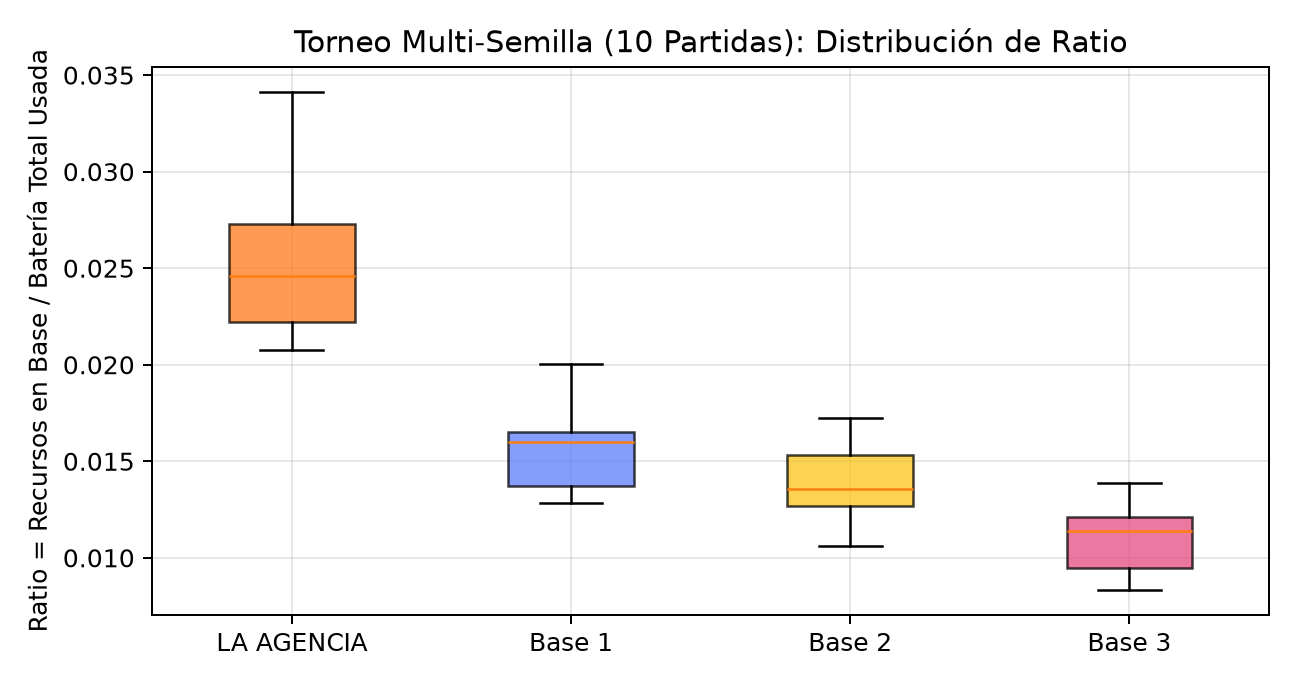
\includegraphics[width=0.70\linewidth]{figuras/torneo_ratio.png}
  \caption{Distribución de la métrica $\text{Ratio}$ en el torneo multi-semilla (10 partidas).}\label{fig:torneo}
\end{figure}

En conclusión, la integración estrictamente descentralizada de memoria con olvido exponencial, utilidad multi-atributo con encadenamiento de vetas y evasión A*, mensajería FIPA-ACL con filtros anti-saturación, subastas CNP y consenso deliberativo tipo AutoGen permite a \textbf{LA AGENCIA} superar consistentemente en $+62.8\,\%$ a los equipos base respetando el presupuesto energético, la integridad arquitectónica y la fluidez gráfica en tiempo real.

\end{document}
